\subsection{Vriendjes} \label{sec:vriendjes}

De directe buren en buren die via een directe buur bekend zijn (via's) worden opgeslagen als een `vriendje' object. Deze vriendjes worden opgeslagen in een simpele array. De array is standaard 253 vriendjes lang. Dit komt omdat elke node een ID heeft van 1 byte, waardoor er 256 mogelijke ID's zijn. In de ISO staat dat de ID's 0x00 en 0xff niet gebruikt mogen worden. Ook zou een node nooit zichzelf moeten opslaan als vriendje. Hierdoor blijven er 253 ID's over.
In \autoref{fig:friendsList} is de werking van de vriendjes array te zien.


\begin{figure}[ht]
    \centering
    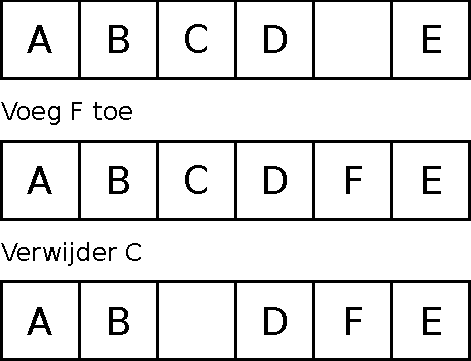
\includegraphics[width=0.45\textwidth]{img/friendList.pdf}
    \caption{Hoe de vriendjes array werkt.}
    \label{fig:friendsList}
\end{figure}

De array is zo gemaakt dat, wanneer een node weggehaald moet worden, zijn ID gewoon naar 0 gezet kan worden. Wanneer het ID van een van de vriendjes in de array 0 is, wordt deze genegeerd door de code. Wanneer er een nieuw vriendje toe wordt gevoegd, word deze op de eerst mogelijke positie gezet waar het ID gelijk is aan 0. Op deze manier hoeft de array niet elke keer opgeschoven te worden wanneer er een vriendje weggehaald wordt.

Er zijn 2 soorten vriendjes: een direct vriendje en een via. Deze worden in hetzelfde datatype in dezelfde array opgeslagen. Elk vriendje bevat de volgende data:
\begin{description}
    \item[ID]       Het ID van het vriendje.
    \item[Hops]     In hoeveel hops het vriendje bekend is.
    \item[Via]      Via welk directe vriendje dit vriendje bekend is.
    \item[Vertrouwen]    Hoe betrouwbaar een direct vriendje is.
    \item[Actief]   Of het vriendje betrouwbaar genoeg is om berichten naar te kunnen sturen.
\end{description}

De Vertrouwen en Actief eigenschappen zijn bedoeld voor directe vriendjes. Wanneer een node A een snapshot ontvangt van een vriendje B, zal node A het vertrouwen van B met twee ophogen. Wanneer node A zelf een snapshot stuurt verlaagt hij het vertrouwen van al zijn vriendjes met één. Op deze manier zal er consequent elke periode een snapshot ontvangen moeten worden om het vertrouwen te verhogen. Wanneer het vertrouwen boven 5 uitkomt, zal de node actief gemaakt worden. Dat wil zeggen dat het vriendje nu genoeg vertrouwd wordt om er data naartoe te sturen en om hem te gebruiken als bron van via's. Wanneer het vertrouwen onder 5 valt zal het vriendje niet meer actief gemaakt worden. Het vertrouwen zal nooit boven de 7 uitkomen. Deze waardes (5 en 7) zijn een inschatting, en er zou meer getest moeten worden om te bevestigen of ze ideaal zijn voor onze doeleinden.


\begin{figure}[ht]
    \centering
    \begin{tikztimingtable}
        B Actief            & 19L 1S 3L 9H 4L \\
        Vertrouwen van B    & 3D{0} 1D{2} 4D{1} 3D{0} 1D{2} 3D{1} 1D{3} 3D{2} 1S 3D{5} 1D{7} 4D{6} 4D{5} 4D{4} \\
        Snapshot van B      & 3L G 8L G 4L G 4L 1S 3L G 13L \\
        Snapshot door A     & 4L G 4L G 4L G 4L G 3L 1S 4L G 4L G 4L G 4L\\
    \end{tikztimingtable}
    \caption{Een voorbeeld van hoe het vertrouwenssysteem werkt, gezien vanuit node A.}
    \label{fig:trustSystem}
\end{figure}

De Hops en Via eigenschappen zijn bedoeld voor de vriendjes die via een ander, direct vriendje bekend zijn. Deze via's worden toegevoegd wanneer een actief vriendje een snapshot stuurt met vriendjes-data er in, van vriendjes die wij nog niet kennen. In een via vriendje wordt opgeslagen in hoeveel hops hij te bereiken is (dit wordt in de snapshot meegestuurd), en via wie hij bekend is (het actieve vriendje waarvan de snapshot is ontvangen). Wanneer een via vriendje plotseling wel direct te bereiken is, wordt het vertrouwen nog steeds opgehoogd. Wanneer het vriendje actief wordt, worden de Via en Hop data van het vriendje verwijderd. Dit wordt gedaan om de situatie in \autoref{fig:HopsOpslaanVanActieveNode} te voorkomen.


\begin{figure}[ht]
    \centering
    \begin{subfigure}[][4cm][t]{0.8\textwidth}
        \centering
        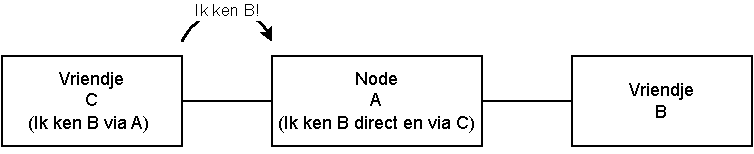
\includegraphics[scale=1]{img/incorrectAssumption.pdf}
        \caption{Een incorrecte aanname van A.}
        \label{fig:incorrectAssumption}
    \end{subfigure}
    \hfill
    \begin{subfigure}{0.8\textwidth}
        \centering
        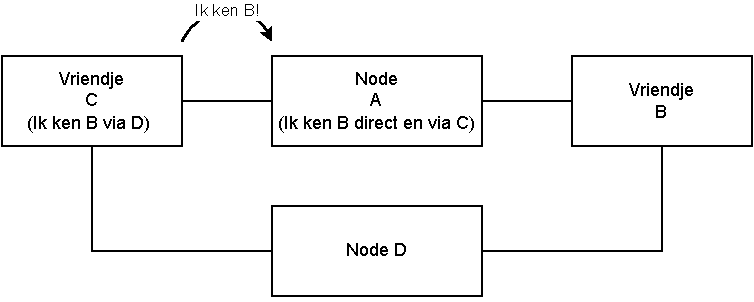
\includegraphics[scale=1]{img/correctAssumption.pdf}
        \caption{Een correcte aanname van A.}
        \label{fig:correctAssumption}
    \end{subfigure}
    \caption{Twee situaties waarin node A exact dezelfde informatie ontvangt, waar node A hops en via informatie blijft opslaan van nodes die hij direct kent.}
    \label{fig:HopsOpslaanVanActieveNode}
\end{figure}